\section{Variable Name Generation Model}
\label{sec:name-gen}

\begin{figure*}[ht]
	\begin{center}
	  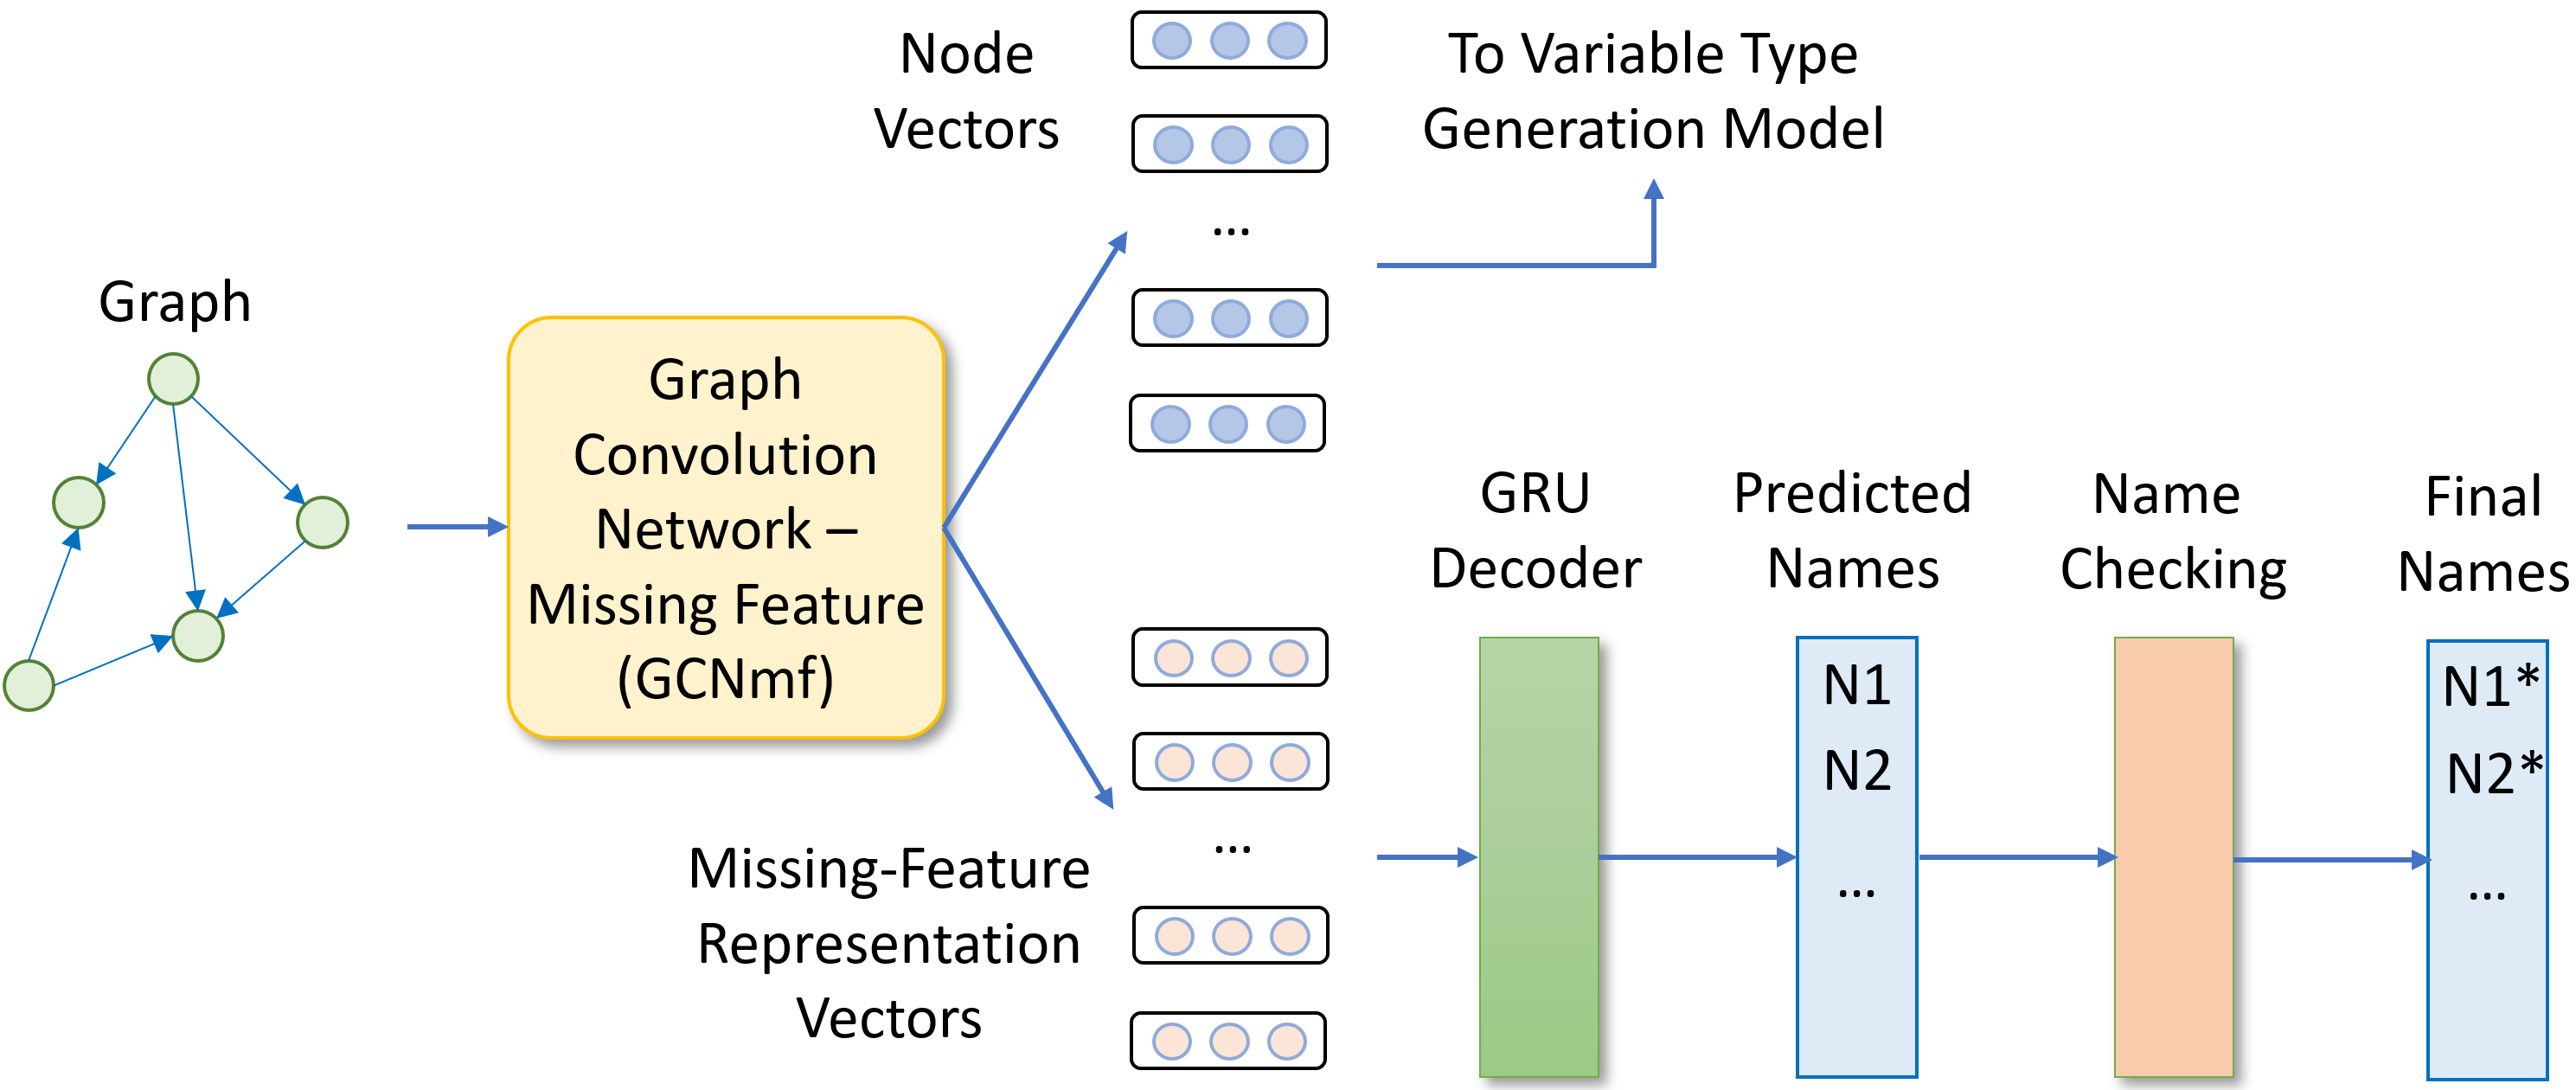
\includegraphics[width=5.7in]{figures/name-gen-model}
          \vspace{-6pt}
		\caption{The Variables Name Generation Model (VNG)}
		\label{fig:name-gen}
	\end{center}
\end{figure*}

1> Similar to step 2, we use GloVe to learn the representation vector.

2> For the node that represent the variable with minified name, we mask the node feature and regard it as the missing feature.

3> Put the graph with missing feature for some nodes into the $GCN_{mf}$ as input. 

4> The $GCN_{mf}$ can output the predicted missing node feature representation vector $V_{rm}$ and the node representation vector $V'_r$. The node representation vector $V'_r$ will be used in step 2.

5> Use $V_{rm}$ as the input of a GRU (RNN) decoder, and the decoder generate the names for the variables with the minified name.

6> When doing generation, we apply basic checking to make sure the same variable has only one consistent name.


Multi-task learning

We use the uncertainty weighted multi-task loss as the multitask learning loss function and use the maximum of the top-1 accuracy score from two tasks as the training target.
